\section{Классификация белков по функции. Ферменты, классификация ферментов (примеры для основных групп по EC - «Enzyme Commission»/«классификация ферментов»). Хроматографические методы разделения белков: гель-фильтрация, ионообменная хр-я, обращённая фаза, аффинная хр-я.}

\subsection{Функции белков:}

\begin{enumerate}
	\item \textbf{строительная} -- белки участвуют в образовании клеточных и внеклеточных структур (например, белки клеточных мембран);
	
	\item \textbf{транспортная} -- некоторые белки способны присоединять различные вещества и переносить их из одного места клетки в другое (например, \textit{гемоглобин} осуществляет транспорт кислорода);
	
	\item \textbf{регуляционная} -- осуществление регуляции процессов в клетке (например, факторы транскрипции);
	
	\item \textbf{защитная} -- белки имунной защиты (антитела), химической защиты (ферменты печени), физической защиты (\textit{фибриноген} опеспечивает свертываемость крови);
	
	\item \textbf{двигательная} -- сократительные белки актин и миозин обеспечивают сокращение мышц у многоклеточных животных, движений листьев у растений, мерцание ресничек у простейших и т.д.;
	
	\item \textbf{сигнальная} -- в поверхностную мембрану клетки встроены молекулы белков (рецепторы), способных изменять свою третичную структуру в ответ на действие факторов внешней среды, таким образом осуществляя прием сигналов из внешней среды и передачу команд в клетку (например, \textit{адренорецептор} сообщает клетке о присоединении адреналина);
	
	\item \textbf{запасающая} -- казалось бы, клетка питается не белками, но в условиях острого голода, когда ну совсем больше ничего нет, можно и их покушать. У животных и человека при длительном голодании используются белки мышц, эпителиальных тканей и печени. Кажется, \textit{E. coli} умеет кушать свои рибосомы.
	
	\item \textbf{каталитическая} -- или ферментативная (например, \textit{ДНК-полимераза} синтезирует ДНК);
	
	\item \textbf{трофическая} -- близка к транспортной, но не она. Почему-то выделяют в отдельную группу. Основной пример - белок молока (казеин) питает новорожденных. Либо выделяют эту функцию как питание зародышей (например, так делает белок \textit{ихтулин} рыбьей икры).
\end{enumerate}

\subsection{Классификация ферментов:}

\begin{itemize}
	\item \textbf{EC1} -- \textit{оксиредуктаза} -- катализирует перенос электронов, то есть окисление или восстановление. Например, фермент \textit{каталаза} способствует разложению пероксида водорода: \ce{2H2O2 -> 2H2O + O2};
	
	\item \textbf{EC2} -- \textit{трансфераза} -- катализирует перенос функциональных групп и молекулярных остатков от одной молекулы к другой. Например, фермент \textit{гексокиназа} перевешивает фосфат с АТФ на шестой углерод глюкозы:
	\begin{equation*}
	\text{глюкоза + АТФ} \ce{->} \text{глюкозо-6-фосфат + АДФ};
	\end{equation*}
	
	\item \textbf{EC3} -- \textit{гидролаза} -- катализирует гидролиз ковалентной связи. Например, фермент \textit{карбоксипептидаз} гидролизует пептидную связь: 
	\begin{figure}[H]
		\centering
		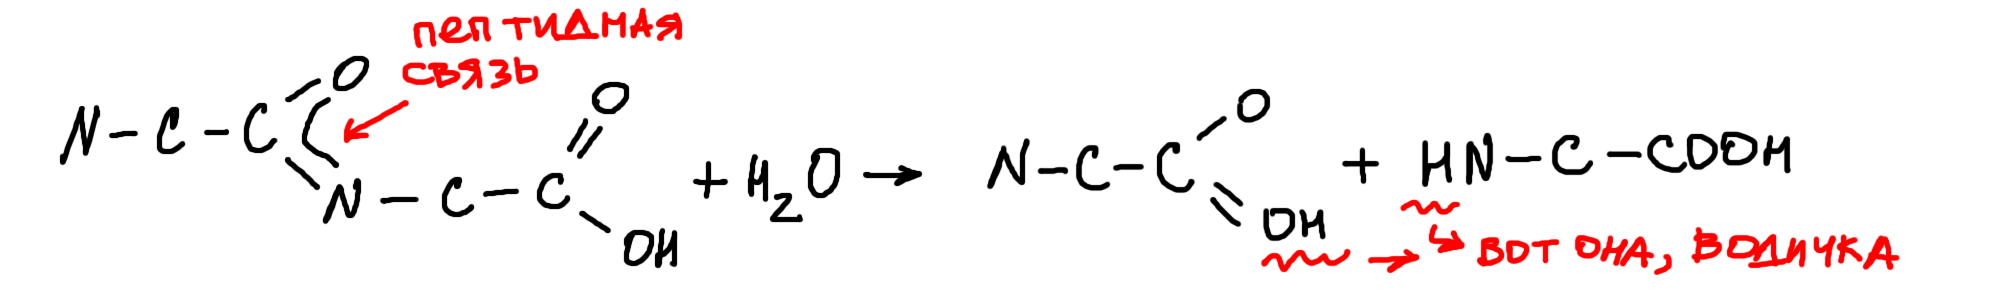
\includegraphics[width=\linewidth]{Pictures/Hydrolase.jpg}
		\caption{Гидролиз пептидной связи карбоксипептидазой.}
	\end{figure}

	\item \textbf{EC4} -- \textit{лиаза} -- катализирует реакции негидролитического и неокислительного разрыва различных химических связей (разрывает связи, но не присоединяет воду). Например, фермент \textit{метионин-$\gamma$-лиаза} катализирует разложение метионина:
		\begin{figure}[H]
		\centering
		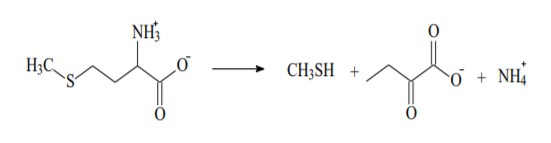
\includegraphics[width=\linewidth]{Pictures/Lease.jpg}
		\caption{Реакция $\gamma$-разложения метионина лиазой.}
	\end{figure}

	\item \textbf{EC5} -- \textit{изомераза} -- катализирует структурные превращения изомеров. Например, фермент \textit{фосфоглюкозоизомераза} делает из глюкозы-6-фосфата фруктозу-6-фосфат:
	\begin{figure}[H]
		\centering
		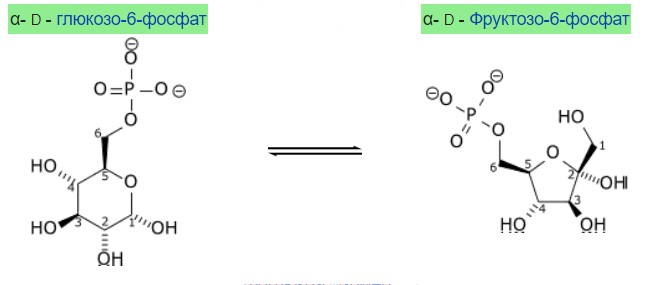
\includegraphics[width=\linewidth]{Pictures/Izomerase.jpg}
		\caption{Превращение глюкозы с фосфатом во фруктозу с фосфатом (одна из реакций гликолиза).}
	\end{figure}

	\item \textbf{EC6} -- \textit{лигаза} -- катализирует соединение двух молекул с образованием новой химической связи — лигирование. Например, фермент \textit{ДНК-лигаза} способствует образованию фосфодиэфирных связей между 5'- и 3'-концами соседних нуклеотидов в ДНК (важный процесс -- лигирование фрагментов Оказаки при репликации ДНК).
\end{itemize}

\subsection{Хроматографические методы разделения белков}
Смесь растворенных белков пропускают через колонку (полую стеклянную трубку, суженую к низу, как перевернутая бутылка), наполненную маленкими твердыми пористыми шариками. Проходя через такую систему, некоторые белки попадают в поры шариков и задерживаются в них. В зависимости от свойств шариков происходит разделение белков по различным параметрам (см. рисунки!):

\begin{itemize}
	\item \textbf{гель-фильтрация} -- разделение по размеру -- белки маленького размера удершиваются в пористых шариках, а белки большого размера в них не пролезают и просто смываются из колонки;
	
	\item \textbf{ионообменная хроматография} -- разделение по заряду -- наполним колонку заряженными шариками, тогда белки, заряженные противоположно будут притягиваться к шарикам, и чем больше заряд, тем сильнее они удерживаются в колонке;	
	
	\item \textbf{обращённая фаза} -- разделение по гидрофобности/гидрофильности -- интересно, как насыпать в жижу гидрофобных шариков, чтоб они между собой не слиплись? Короче, используется нечто, притягивающее гидрофобные белки. Гидрофильные, ни с чем ни связанные, смываются;
	
	\item \textbf{аффинная хроматография} -- разделение по способности связывать определенный вид молекул -- очевидно, наполнитель из этих самых молекул.
	
	\begin{figure}[H]
	\centering
	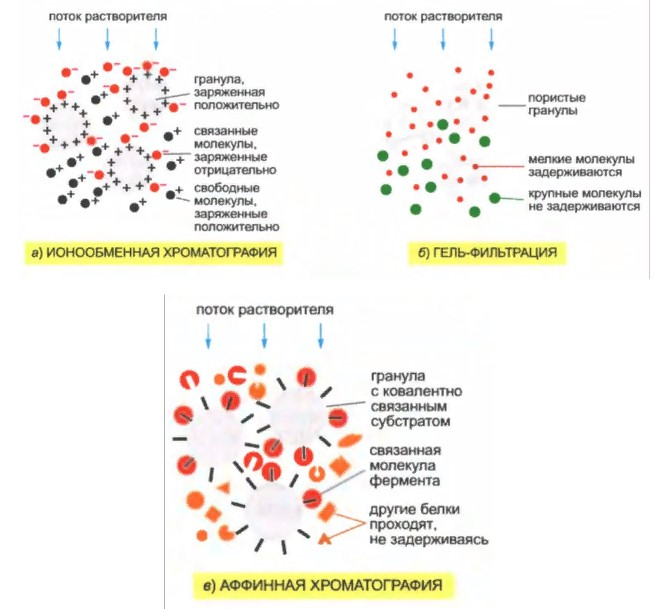
\includegraphics[width=\linewidth]{Pictures/Cromato.jpg}
	\caption{Различные виды хроматографии наглядно.}
\end{figure}
\end{itemize}
